\documentclass{beamer}

\pdfmapfile{+sansmathaccent.map}


\mode<presentation>
{
	\usetheme{Warsaw} % or try Darmstadt, Madrid, Warsaw, Rochester, CambridgeUS, ...
	\usecolortheme{seahorse} % or try seahorse, beaver, crane, wolverine, ...
	\usefonttheme{serif}  % or try serif, structurebold, ...
	\setbeamertemplate{navigation symbols}{}
	\setbeamertemplate{caption}[numbered]
} 


%%%%%%%%%%%%%%%%%%%%%%%%%%%%
% itemize settings


%%%%%%%%%%%%%%%%%%%%%%%%%%%%
% itemize settings

\definecolor{myhotpink}{RGB}{255, 80, 200}
\definecolor{mywarmpink}{RGB}{255, 60, 160}
\definecolor{mylightpink}{RGB}{255, 80, 200}
\definecolor{mypink}{RGB}{255, 30, 80}
\definecolor{mydarkpink}{RGB}{155, 25, 60}

\definecolor{mypaleblue}{RGB}{240, 240, 255}
\definecolor{mylightblue}{RGB}{120, 150, 255}
\definecolor{myblue}{RGB}{90, 90, 255}
\definecolor{mygblue}{RGB}{70, 110, 240}
\definecolor{mydarkblue}{RGB}{0, 0, 180}
\definecolor{myblackblue}{RGB}{40, 40, 120}

\definecolor{mygreen}{RGB}{0, 200, 0}
\definecolor{mygreen2}{RGB}{245, 255, 230}

\definecolor{mygray}{gray}{0.8}
\definecolor{mydarkgray}{RGB}{80, 80, 160}

\definecolor{mydarkred}{RGB}{160, 30, 30}
\definecolor{mylightred}{RGB}{255, 150, 150}
\definecolor{myred}{RGB}{200, 110, 110}
\definecolor{myblackred}{RGB}{120, 40, 40}

\definecolor{mygreen}{RGB}{0, 200, 0}
\definecolor{mygreen2}{RGB}{205, 255, 200}

\definecolor{mydarkcolor}{RGB}{60, 25, 155}
\definecolor{mylightcolor}{RGB}{130, 180, 250}

\setbeamertemplate{itemize items}[default]

\setbeamertemplate{itemize item}{\color{myblackblue}$\blacksquare$}
\setbeamertemplate{itemize subitem}{\color{mygblue}$\blacktriangleright$}
\setbeamertemplate{itemize subsubitem}{\color{mygray}$\blacksquare$}

\setbeamercolor{palette quaternary}{fg=white,bg=mydarkgray}
\setbeamercolor{titlelike}{parent=palette quaternary}

\setbeamercolor{palette quaternary2}{fg=black,bg=mypaleblue}
\setbeamercolor{frametitle}{parent=palette quaternary2}

\setbeamerfont{frametitle}{size=\Large,series=\scshape}
\setbeamerfont{framesubtitle}{size=\normalsize,series=\upshape}





%%%%%%%%%%%%%%%%%%%%%%%%%%%%
% block settings

\setbeamercolor{block title}{bg=red!30,fg=black}

\setbeamercolor*{block title example}{bg=mygreen!40!white,fg=black}

\setbeamercolor*{block body example}{fg= black, bg= mygreen2}


%%%%%%%%%%%%%%%%%%%%%%%%%%%%
% URL settings
\hypersetup{
	colorlinks=true,
	linkcolor=blue,
	filecolor=blue,      
	urlcolor=blue,
}

%%%%%%%%%%%%%%%%%%%%%%%%%%

\renewcommand{\familydefault}{\rmdefault}

\usepackage{amsmath}
\usepackage{mathtools}

\usepackage{subcaption}

\usepackage{qrcode}

\DeclareMathOperator*{\argmin}{arg\,min}
\newcommand{\bo}[1] {\mathbf{#1}}

\newcommand{\R}{\mathbb{R}} 
\newcommand{\T}{^\top}     

\newcommand{\dx}[1] {\dot{\mathbf{#1}}}
\newcommand{\ma}[4] {\begin{bmatrix}
		#1 & #2 \\ #3 & #4
\end{bmatrix}}
\newcommand{\myvec}[2] {\begin{bmatrix}
		#1 \\ #2
\end{bmatrix}}
\newcommand{\myvecT}[2] {\begin{bmatrix}
		#1 & #2
\end{bmatrix}}


\newcommand{\mydate}{Spring 2023}

\newcommand{\mygit}{\textcolor{blue}{\href{https://github.com/SergeiSa/Control-Theory-Slides-Spring-2023}{github.com/SergeiSa/Control-Theory-Slides-Spring-2023}}}

\newcommand{\myqr}{ \textcolor{black}{\qrcode[height=1.5in]{https://github.com/SergeiSa/Control-Theory-Slides-Spring-2023}}
}

\newcommand{\myqrframe}{
	\begin{frame}
		\centerline{Lecture slides are available via Github, links are on Moodle}
		\bigskip
		\centerline{You can help improve these slides at:}
		\centerline{\mygit}
		\bigskip
		\myqr
	\end{frame}
}


\newcommand{\bref}[2] {\textcolor{blue}{\href{#1}{#2}}}

%%%%%%%%%%%%%%%%%%%%%%%%%%%%
% code settings

\usepackage{listings}
\usepackage{color}
% \definecolor{mygreen}{rgb}{0,0.6,0}
% \definecolor{mygray}{rgb}{0.5,0.5,0.5}
\definecolor{mymauve}{rgb}{0.58,0,0.82}
\lstset{ 
	backgroundcolor=\color{white},   % choose the background color; you must add \usepackage{color} or \usepackage{xcolor}; should come as last argument
	basicstyle=\footnotesize,        % the size of the fonts that are used for the code
	breakatwhitespace=false,         % sets if automatic breaks should only happen at whitespace
	breaklines=true,                 % sets automatic line breaking
	captionpos=b,                    % sets the caption-position to bottom
	commentstyle=\color{mygreen},    % comment style
	deletekeywords={...},            % if you want to delete keywords from the given language
	escapeinside={\%*}{*)},          % if you want to add LaTeX within your code
	extendedchars=true,              % lets you use non-ASCII characters; for 8-bits encodings only, does not work with UTF-8
	firstnumber=0000,                % start line enumeration with line 0000
	frame=single,	                   % adds a frame around the code
	keepspaces=true,                 % keeps spaces in text, useful for keeping indentation of code (possibly needs columns=flexible)
	keywordstyle=\color{blue},       % keyword style
	language=Octave,                 % the language of the code
	morekeywords={*,...},            % if you want to add more keywords to the set
	numbers=left,                    % where to put the line-numbers; possible values are (none, left, right)
	numbersep=5pt,                   % how far the line-numbers are from the code
	numberstyle=\tiny\color{mygray}, % the style that is used for the line-numbers
	rulecolor=\color{black},         % if not set, the frame-color may be changed on line-breaks within not-black text (e.g. comments (green here))
	showspaces=false,                % show spaces everywhere adding particular underscores; it overrides 'showstringspaces'
	showstringspaces=false,          % underline spaces within strings only
	showtabs=false,                  % show tabs within strings adding particular underscores
	stepnumber=2,                    % the step between two line-numbers. If it's 1, each line will be numbered
	stringstyle=\color{mymauve},     % string literal style
	tabsize=2,	                   % sets default tabsize to 2 spaces
	title=\lstname                   % show the filename of files included with \lstinputlisting; also try caption instead of title
}


%%%%%%%%%%%%%%%%%%%%%%%%%%%%
% URL settings
\hypersetup{
	colorlinks=false,
	linkcolor=blue,
	filecolor=blue,      
	urlcolor=blue,
}

%%%%%%%%%%%%%%%%%%%%%%%%%%

%%%%%%%%%%%%%%%%%%%%%%%%%%%%
% tikz settings

\usepackage{tikz}
\tikzset{every picture/.style={line width=0.75pt}}


\title{Introduction, ODE and State Space}
\subtitle{Control Theory, Lecture 1}
\author{by Sergei Savin}
\centering
\date{\mydate}



\begin{document}
\maketitle


%\begin{frame}{Content}
%
%\begin{itemize}
%\item Motivation
%\item Ordinary differential equations
%    \begin{itemize}
%    \item 1st order
%    \item n-th order
%    \end{itemize}
%\item Linear differential equations
%    \begin{itemize}
%    \item 1st order
%    \item n-th order
%    \end{itemize}
%\item Changing n-th order ODE to a State-Space form
%\item State-Space to ODE
%\item Read more
%\end{itemize}
%
%\end{frame}



\begin{frame}{What is control?}
% \framesubtitle{O}
\begin{flushleft}

The first obvious question is, what is control theory? The easiest strategy to answer this question is to bring examples of systems that you can \emph{learn how to control}:

\begin{figure}
\minipage{0.45\textwidth}
  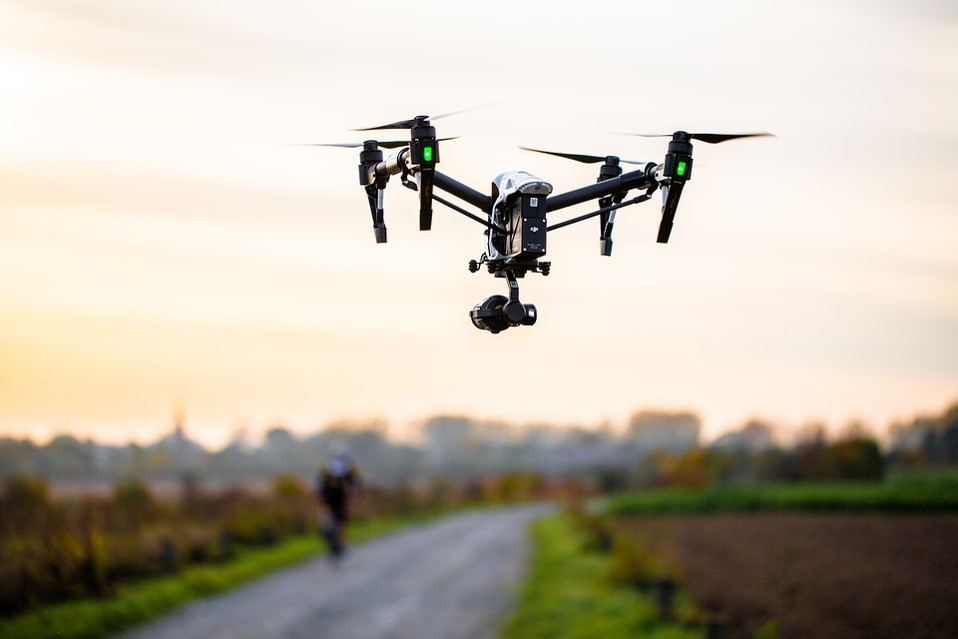
\includegraphics[width=\linewidth]{Picture1.jpg}
  \caption{Drones}
\endminipage\hfill
\minipage{0.45\textwidth}
  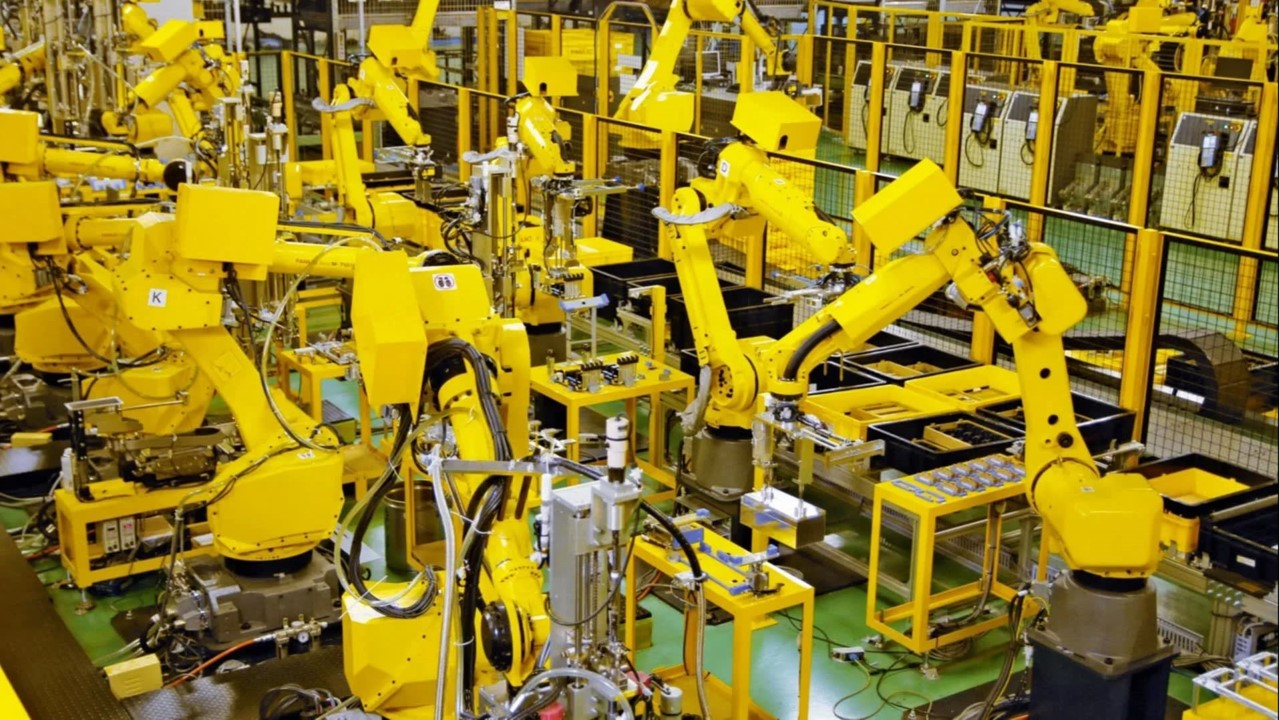
\includegraphics[width=\linewidth]{Picture2.jpg}
  \caption{Industrial robot arms}
\endminipage

\end{figure}

But beware, this is not the whole answer!

\end{flushleft}
\end{frame}



\begin{frame}{Why Control?}
% \framesubtitle{Part 1}
\begin{flushleft}

The second most natural question to ask is - why do we need to study Control Theory?

\bigskip

\begin{exampleblock}{The easy answer is:}
Control is one of the fundamental aspects of Robotics, together with Mechanical and Electrical Engineering, Sensing, Software development, etc.
\end{exampleblock}

A lot of typical practical issues occurring in robotics (such as lag and delays, lack of sensory data, external disturbances, robot having dynamics slightly different from the expected, etc.) are addressed in control theory; you need to understand the topic top be able to use solutions that control theory gives us.

\end{flushleft}
\end{frame}


%\begin{frame}{Control as an applied problem}
%\begin{flushleft}
%
%We propose to view Control Theory as not only yet-another-subject. Instead we can try to see Control Theory course as \textbf{an application of your combined skills as a CS student}
%
%\end{flushleft}
%\end{frame}


%\begin{frame}{Control as an applied problem}
%\framesubtitle{Skills you will learn and practice}
%\begin{flushleft}
%
%In this course we provide you with learning and practical tasks that require:
%
%\begin{itemize}
%    \item Linear Algebra, Differential Equations, Computational methods
%    \item Dynamical systems, Stability (concept build on top of Theory of Ordinary Differential Equations).
%    % \item Linear dynamical systems (a deep look into one of the most useful and reach in scientific results areas of dynamical systems theory)
%    
%    \item Simulation of dynamical systems (closely related to computational methods in Differential Equations), as a programming problem.
%    \item Development of experiments in Google Colab, using Python, mathematical libraries, solving concrete, real world-related math-oriented problems.
%    
%    \item Representation (parametrization) of equations as a tool in both mathematical analysis and simulation, software development and problem solving.
%    
%    \item ...and many other things.
%\end{itemize}
%
%\end{flushleft}
%\end{frame}


%\begin{frame}{...so, why Control?}
%% \framesubtitle{Part 1}
%\begin{flushleft}
%
%Control Theory, as given here, is focused on:
%
%\begin{enumerate}
%    \item Giving you a challenge to simultaneously learn a new concepts, new general and subject-specific math, and new programming tools.
%    \item Providing you with clear outcomes in terms of \emph{understanding} and ability to \emph{solve well-defined and meaningful real-world problems}.
%    \item Being very useful for those who will proceed to work in robotics, automation, self-driving vehicles, drones, etc.
%\end{enumerate}
%
%See it as a test case for your abilities as a CS specialist.
%
%\end{flushleft}
%\end{frame}



\begin{frame}{Enough for the motivation}
% \framesubtitle{Part 1}
\begin{flushleft}


\begin{exampleblock}{Now that we know (kinda) why we do it:}

\hfill \break
Let's start with the content of the course!
\newline

\end{exampleblock}

\end{flushleft}
\end{frame}




\begin{frame}{Ordinary differential equations}
\framesubtitle{1st order}
\begin{flushleft}

Let us remember the normal form of first-order \emph{ordinary differential equations (ODEs):}

\begin{equation}
    \dot{\bo{x}} = \bo{f} (\bo{x}, t)
\end{equation}

where $\bo{x} = \bo{x}(t)$ is the solution of the equation and $t$ is a free variable (usually - time).

\bigskip

\begin{definition}
We can call this equation (same as any other ODEs) a \emph{dynamical system}, and $\bo{x}$ is called the \emph{state} of the dynamical system.  
\end{definition}

\begin{example}
\begin{equation}
    \dot{x} = -3 x^3 - 7 
\end{equation}
\end{example}

\end{flushleft}
\end{frame}




\begin{frame}{State}
%	\framesubtitle{1st order}
	\begin{flushleft}
		
		\emph{State} of a dynamical system is a minimal set of variables that describe the system, in the sense that knowing current state and all future inputs you can predict the behavior of the system.
		
		\begin{example}
			For a spring-damper system, the state variables could be position and velocity of the mass.
		\end{example} 
		\begin{example}
			For a double pendulum, the state variables could be joint angles and joint velocities.
		\end{example} 
		
	\end{flushleft}
\end{frame}






\begin{frame}{Ordinary differential equations, n-th order}
%\framesubtitle{n-th order}
\begin{flushleft}

The normal form of an \emph{n-th order} ordinary differential equation is:

\begin{equation}
	x^{(n)} = f (x^{(n-1)}, x^{(n-2)}, ...\,, \ddot{x}, \dot{x}, x, t)
\end{equation}
			
where $x = x(t)$ is the solution of the equation. Same as before, it is a \emph{dynamical system}, but this time we need more variables to describe the state of this system, for example we can use the set $\{ x, \ \dot{x} , ...\,,x^{(n-1)} \}$.

\begin{example}
\begin{equation}
    \ddot{x} = \cos(2\dot{x}) - 10 x + 7 
\end{equation}
\end{example}


\begin{example}
\begin{equation}
\begin{cases}
    \dddot{x}_1 = \dot{x}_1 + x_1 + x_2^2 - 4 \\
    \dddot{x}_2 = 10 x_1^3 + \ddot{x}_2
\end{cases}
\end{equation}
\end{example}

\end{flushleft}
\end{frame}




\begin{frame}{Linear differential equations}
\framesubtitle{1st order}
\begin{flushleft}

Linear ODEs of the first order have normal form:

\begin{equation}
    \dot{\bo{x}} = \bo{A} \bo{x}
\end{equation}

\begin{example}
\begin{equation}
\begin{cases}
    \dot{x}_1 = -20 x_1 + 7 x_2 \\
    \dot{x}_2 = 10.5 x_1 - 3 x_2
\end{cases}
\end{equation}
\end{example}

\begin{example}
\begin{equation}
\begin{bmatrix}
\dot{x}_1 \\
\dot{x}_2 \\
\dot{x}_3
\end{bmatrix} 
= 
\begin{bmatrix}
-8   & 5   & 2  \\
 0.5 & -10 & -2 \\
 1   & -1 & -20
\end{bmatrix}
\begin{bmatrix}
x_1 \\
x_2 \\
x_3
\end{bmatrix} 
\end{equation}
\end{example}

\end{flushleft}
\end{frame}




\begin{frame}{Linear differential equations, n-th order}
%\framesubtitle{n-th order}
\begin{flushleft}

A single linear ODE of the n-th order are often written in the form:

\begin{equation}
    a_n x^{(n)} + 
    ... +
    a_2 \ddot{x} + a_1 \dot{x} + 
    a_0 x = 0
\end{equation}

\begin{example}
\begin{equation}
12 \dddot{x} -
    3 \ddot{x} + 5.5 \dot{x} + 
    2 x = 0
\end{equation}
\end{example}

\begin{example}
\begin{equation}
    5 \ddot{x} - 2 \dot{x} + 
    10 x = 0
\end{equation}
\end{example}

\end{flushleft}
\end{frame}




\begin{frame}{Equations with an input}
	%\framesubtitle{n-th order}
	\begin{flushleft}
		
		Sometimes it is convenient to write an ODE in the form with an \emph{input}, for example:
		
		\begin{equation}
			a_2 \ddot{x} + a_1 \dot{x} + 
			a_0 x = u(t)
		\end{equation}
		
		In this equation $u(t)$ is a function of time. This form offers us many uses:
		
		\begin{itemize}
			\item We can use $u(t)$ to model \emph{control input}, (e.g. voltage, motor torque) that we directly control.
			
			\item We can use $u(t)$ to model external forces acting on the system.
			
			\item We can substitute particular function instead of $u(t)$, e.g. sine wave or step function, to study how the system behaves with such an input.
		\end{itemize}
		
	\end{flushleft}
\end{frame}



\begin{frame}{Equations with an input}
	%\framesubtitle{n-th order}
	\begin{flushleft}
		
		General form of an n-th order linear ODE with an input can be presented as follows:
		%
		\begin{equation}
			a_n x^{(n)} + 
			... +
			a_2 \ddot{x} + a_1 \dot{x} + 
			a_0 x = u(t)
		\end{equation}
	
	\bigskip
		
		State-space representation of a linear system with an input is:
		%
		\begin{equation}
			\dot{\bo{x}} = \bo{A} \bo{x} + \bo{B} \bo{u}
		\end{equation}
		
		
	\end{flushleft}
\end{frame}







\begin{frame}{Equations with an output}
	%\framesubtitle{n-th order}
	\begin{flushleft}
		
		Equations can also have an output. The meaning of what is an output of an equation depends on the particular use-case - it is not a mathematical issue, it is a question of interpretation. For example, an output can mean:
		
		\begin{itemize}
			\item What we measure (height of a quadrotor, angular velocity of motor's rotor, etc.).
			
			\item We care about and/or what we can to control (position and orientation of a quadrotor, velocity of a car, etc.)
			
			\item etc.
		\end{itemize}
		
		We often denote output as $y$, and it depends on the state of the system: $y = g(\bo{x})$
		
	\end{flushleft}
\end{frame}


\begin{frame}{Equations with an output}
	%\framesubtitle{n-th order}
	\begin{flushleft}
		
		State-space representation of a linear system with an input and an output is:
		%
		\begin{equation}
		\begin{cases}
				\dot{\bo{x}} = \bo{A} \bo{x} + \bo{B}\bo{u} \\
				\bo{y} = \bo{C}\bo{x}
		\end{cases}
		\end{equation}
		
		If $\bo{u} \in \R$ and $\bo{y} \in \R$ (i.e. if they are scalars) and you want to represent the system with an output as a single ODE, it is typical to treat the output as ODE the variable:
		
		\begin{equation}
			a_n y^{(n)} + 
			... +
			a_2 \ddot{y} + a_1 \dot{y} + 
			a_0 y = u(t)
		\end{equation}
		
	\end{flushleft}
\end{frame}






\begin{frame}{Linear differential equations}
%\framesubtitle{...are what we will study}
\begin{flushleft}

In this course we will focus entirely on linear dynamical systems. In particular, we will take a good use of the following two forms:

\begin{equation}
    a_n y^{(n)} +
    ... +
    a_2 \ddot{y} + a_1 \dot{y} + 
    a_0 y = u(t)
\end{equation}

\begin{equation}
	\begin{cases}
		\dot{\bo{x}} = \bo{A} \bo{x} + \bo{B}\bo{u} \\
		\bo{y} = \bo{C}\bo{x}
	\end{cases}
\end{equation}

the last one is called \emph{state-space representation}. In general both $\bo{u}$ and $\bo{y}$ can be vectors.

\begin{exampleblock}{Good news:}

\hfill \break
Both of those can be used to express any linear system, hence we can change one into the other.
\newline

\end{exampleblock}

\end{flushleft}
\end{frame}




\begin{frame}{n-th order ODE to State-Space}
% \framesubtitle{...are what we will study}
\begin{flushleft}

Consider eq. $\dddot{y} + a_2 \ddot{y} + a_1 \dot{y} + a_0 y =u$.

\bigskip

Make a substitution: $x_1 = y$, $x_2 = \dot{y}$, $x_3 = \ddot{y}$. Therefore:

\begin{equation}
    \begin{cases}
        \dot{x}_1 = \dot{y} = x_2 \\
        \dot{x}_2 = \ddot{y} = x_3 \\
        \dot{x}_3 =  u-a_2 \ddot{y} - a_1 \dot{y} - a_0 y = 
        u-a_2 x_3 - a_1 x_2 - a_0 x_1
    \end{cases}
\end{equation}

Which can be directly put in the state-space form:

\begin{equation}
\begin{bmatrix}
\dot{x}_1 \\ \dot{x}_2 \\ \dot{x}_3
\end{bmatrix} 
=
\begin{bmatrix}
0 & 1 & 0 \\ 
0 & 0 & 1 \\
-a_0 & -a_1 & -a_2
\end{bmatrix} 
\begin{bmatrix}
x_1 \\ x_2 \\ x_3
\end{bmatrix} 
+ 
\begin{bmatrix}
0 \\ 0 \\ u
\end{bmatrix}
\end{equation}


\end{flushleft}
\end{frame}



\begin{frame}{State Space to ODE}
\centerline{An example of how linear algebra serves}
\centerline{to solve a seemingly difficult problem}
\bigskip
\centerline{(advanced, not going to be on the test)}
\end{frame}




\begin{frame}{State Space to ODE}
\begin{flushleft}

Consider a system in state-space form:

\begin{equation}
	\label{eq:SS}
	\begin{cases}
		\begin{bmatrix}
			\dot x_1 \\ 
			\dot x_2
		\end{bmatrix} 
		 = 
		\begin{bmatrix}
			a_{11} & a_{12} \\ 
			a_{21} & a_{22}
		\end{bmatrix} 
\begin{bmatrix}
	x_1 \\ 
	x_2
\end{bmatrix} 
		 \\
		y = 
		\begin{bmatrix}
			c_1 & 
			c_2
		\end{bmatrix} 
	\begin{bmatrix}
	x_1 \\ 
	x_2
\end{bmatrix} 
	\end{cases}
\Longleftrightarrow \ \ 
\begin{cases}
\dx{x} = \bo{A} \bo{x} \\
y = \bo{C} \bo{x} 
\end{cases}
\end{equation}

We want to rewrite it as a linear ODE:

\begin{equation}
\label{eq:ODE}
\ddot{y} + b_2 \dot{y} + b_1 y = 0
\end{equation}

Note that initial conditions of both equation need to agree.


\end{flushleft}
\end{frame}



\begin{frame}{State Space to ODE}
\begin{flushleft}

Since $y = \bo{C} \bo{x}$, its derivative is $\dot y = \bo{C} \dot{\bo{x}}$:

\begin{equation}
\dot y = \bo{C} \bo{A} \bo{x}
\end{equation}
%
\begin{equation}
\dot y = \myvecT{(a_{11}c_1 + a_{21}c_2)}{(a_{12}c_1 + a_{22}c_2)}
\myvec{x_1}{x_2}    
\end{equation}

Analogous for $\ddot y$:

\begin{equation}
\ddot y = \bo{C} \bo{A} \bo{A} \bo{x}
\end{equation}

\end{flushleft}
\end{frame}




\begin{frame}{State Space to ODE}
\begin{flushleft}

Combining our results we find the linear transformation between the variables $x_1$, $x_2$ and $y$, $\dot y$:

\begin{equation}
\myvec{y}{\dot y} = 
\begin{bmatrix}
	c_1                                     & c_2 \\ 
	(a_{11}c_1 + a_{21}c_2) & (a_{12}c_1 + a_{22}c_2)
\end{bmatrix} 
\myvec{x_1}{x_2}    
\end{equation}

Resulting transformation matrix is:

\begin{equation}
\bo{T} = 
\begin{bmatrix}
	c_1                                     & c_2 \\ 
	(a_{11}c_1 + a_{21}c_2) & (a_{12}c_1 + a_{22}c_2)
\end{bmatrix} 
\end{equation}
\begin{equation}
	 \bo{x}
= 
	\bo{T}^{-1}
	\begin{bmatrix}
		y \\ 
		\dot y
	\end{bmatrix} 
\end{equation}

\end{flushleft}
\end{frame}



\begin{frame}{State Space to ODE}
\begin{flushleft}

Remember that:
%
\begin{align}
	\ddot y = \bo{C} \bo{A} \bo{A} \bo{x}
	\\
    \ddot y = \bo{C} \bo{A} \bo{A} \bo{T}^{-1} 
    \begin{bmatrix}
    	y \\ 
    	\dot y
    \end{bmatrix}
\end{align}

So, we obtained $\ddot y$ as a linear function of $y$, $\dot y$.       From this it is clear how the same can be generalized to higher dimensions.

\end{flushleft}
\end{frame}



\begin{frame}{State Space to ODE}
%\framesubtitle{part 5}
\begin{flushleft}

\textcolor{blue}{\href{https://github.com/SergeiSa/Control-Theory-Slides-Spring-2022/blob/main/ColabNotebooks/StateSpace2ODE.ipynb}{Check out the code implementation.}}

\bigskip


\centerline{\textcolor{black}{\qrcode[height=2.1in]{https://github.com/SergeiSa/Control-Theory-Slides-Spring-2022/blob/main/ColabNotebooks/StateSpace2ODE.ipynb}}}


\end{flushleft}
\end{frame}




\begin{frame}{Read more}

\begin{itemize}
	
\item 2.14 Analysis and Design of Feedback Control Systems:

\begin{itemize}
	\item  \bref{http://web.mit.edu/2.14/www/Handouts/StateSpace.pdf}{State-Space Representation of LTI Systems}
	
	\item  \bref{http://web.mit.edu/2.14/www/Handouts/StateSpaceResponse.pdf}{Time-Domain Solution of LTI State Equations}
\end{itemize}	
	
\item \bref{https://lpsa.swarthmore.edu/}{Linear Physical Systems Analysis}:

\begin{itemize}
\item State Space Representations of Linear Physical Systems \bref{https://lpsa.swarthmore.edu/Representations/SysRepSS.html}{lpsa.swarthmore.edu/Representations/SysRepSS.html}

\item Transformation: Differential Equation to State Space \bref{https://lpsa.swarthmore.edu/Representations/SysRepTransformations/DE2SS.html}{lpsa.swarthmore.edu/.../DE2SS.html}
\end{itemize}	

\end{itemize}

\end{frame}



\myqrframe

\end{document}
